\chapter{Rational Reasoning about Spatial and Temporal Relations}
\label{sec:p19-rationality-13-2}

Reasoning from relations between places or events is not the same task as
rotating an object. Ragni's chapter~13.2 compares three levels: qualitative
formalisms supplying idealized correctness conditions; behavioral and neural
evidence concerning people's responses; and computational models proposing
how those responses arise. Its explanation emphasizes a preferred mental
model, limited working memory and the cost of constructing or changing a
representation. A useful first representation can save effort without making
every conclusion drawn from it logically necessary
\cite[pp.~725--733]{Ragni2021SpatialTemporal}.

The treatment retains the source's spatial and temporal examples, interval
table, region-connection distinctions, six behavioral effects, neural
discussion, computational account and rationality argument. Allen's original
propagation procedure, the original PRISM experiments, and a primary
durative-consistency experiment supply bounded supporting records. Neither
an AI relation calculus nor an association between brain activity and a task
is by itself a complete psychological explanation.

\section{Choose the relation, task and standard of success}
\label{sec:p19-rat132-tasks}

\begin{hbdefinition}{def:p19-rat132-task}{Qualitative relation and query type}
A qualitative description groups quantitative states by the relations
relevant to a task, without fixing distances, dates or durations. For a
specified interpretation, let \(\Gamma\) be a finite premise set and let
\(\mathcal M(\Gamma)\) be its satisfying configurations. A consistency
query asks whether this set is nonempty. A possibility query asks whether
some member satisfies the proposed conclusion \(q\). A necessity query asks
whether every member satisfies \(q\). For informative necessity judgments
below, premise satisfiability is checked separately rather than treating
inconsistent premises as an ordinary spatial situation.

A generation task can request one satisfying arrangement, every qualitatively
different arrangement, or a relation common to all arrangements. These
outputs have different correctness conditions. A true feature of one
arrangement answers neither the every-arrangement task nor, by itself, a
necessary-consequence question.
\index{spatial reasoning!preferred models}
\index{temporal reasoning!qualitative relations}
\end{hbdefinition}

In the source's navigation example the reasoner is at a train station; a
bicycle is outside the church's north entrance; and the church is north of
the station. Heading north is justified if the entrance's intrinsic front
is northward and the entities are interpreted in a common north--south
frame. The answer is a direction, not a route, distance, accessibility
guarantee or obstacle-free path. The source notes that an abstract model,
an inference rule or a simple ``use the mentioned cardinal direction''
heuristic all give the same answer here. Agreement on this item cannot
identify which process produced a response. The heuristic fails, for
example, if the bicycle is actually south of the station despite another
premise mentioning north. Intrinsic front, observer-relative front and
cardinal north must not be interchanged without an interpretation
\cite[pp.~725--726]{Ragni2021SpatialTemporal}.

The temporal example says that the complete decoding of the human genome
occurred after the first moon landing, while the computer's invention
occurred before it. Treating these as ordered events gives invention before
decoding. Adding background knowledge may suggest that computers helped the
decoding, but temporal order alone does not imply causal importance. If the
events have relevant duration, a point abstraction must be justified: their
beginnings and endings need not have the same ordering.

\begin{hbtheorem}{thm:p19-rat132-order}{proved=annex:p19.rat132.order}{The source's ordered-event consequence and its causal boundary}
For event points \(c,m,g\) on one strict time order,
\(c<m\) and \(m<g\) imply \(c<g\). These order premises
alone do not imply any causal influence from \(c\) to \(g\).
Likewise, northward transitivity follows from increasing north coordinates
in one fixed frame, not from an arbitrary relation's name.
\end{hbtheorem}

Ragni introduces Kant's account of space and time as a historical framing,
not as an empirical finding establishing a cognitive algorithm. The operative
assumption is that useful reasoning in a complex environment is constrained
by information and cognitive resources. Qualitative compression is useful
when exact information is unavailable or irrelevant; it can lose what a
metrical task needs. ``Earlier'' suffices to order two appointments but does
not establish whether there is enough travel time between them
\cite[secs.~1,7]{Ragni2021SpatialTemporal}.

\section{Interval relations and a bounded formal procedure}
\label{sec:p19-rat132-intervals}

\begin{hbdefinition}{def:p19-rat132-interval}{Proper intervals and the thirteen base relations}
For the endpoint benchmark an interval \(I=(i^-,i^+)\) has real
endpoints with \(i^-<i^+\). This ordered pair describes a positive
duration, not an instantaneous event or a claim about which boundary points
belong to a physical event. Ragni's base symbols are \(b,m,o,d,s,f,e\)
and their inverses \(bi,mi,oi,di,si,fi\), with \(e\) its own
inverse. Table~\ref{tab:p19-rat132-intervals} declares their meanings.
An inverse exchanges the two intervals. A relation set represents
disjunction: \(I\{b,o\}J\) means before \emph{or} overlapping
from the earlier side, not both and not a probability assignment.
\end{hbdefinition}

\begin{table}[htbp]
\centering\small
\begin{tabular}{llll}
Temporal name & Symbol & Endpoint condition & Spatial interval reading\\\hline
before & \(b\) & \(i^+<j^-\) & strictly to the left\\
meets & \(m\) & \(i^+=j^-\) & touches at the left\\
overlaps & \(o\) & \(i^-<j^-<i^+<j^+\) & overlaps from the left\\
during & \(d\) & \(j^-<i^-<i^+<j^+\) & strictly within\\
starts & \(s\) & \(i^-=j^-,\ i^+<j^+\) & left-justified within\\
finishes & \(f\) & \(j^-<i^-,\ i^+=j^+\) & right-justified within\\
equals & \(e\) & \(i^-=j^-,\ i^+=j^+\) & same interval
\end{tabular}
\caption{Endpoint reconstruction of Ragni's Table~13.2.1. The six
asymmetric rows together with their inverses and equality give thirteen
relations. The spatial readings concern intervals on a common axis, not
arbitrary planar regions.}
\label{tab:p19-rat132-intervals}
\end{table}

\begin{hbtheorem}{thm:p19-rat132-endpoints}{proved=annex:p19.rat132.endpoints}{Classification and finite endpoint-order decision}
Exactly one of the thirteen base relations holds between two proper real
intervals. For finitely many such intervals with constraints expressed as
sets of base relations, consistency, possibility and necessity are decidable
by enumerating the weak orders of their finitely many endpoints. Equal
endpoints must remain allowed. Assigning integer ranks to equal-endpoint
classes preserves every base relation. This is a complete procedure for the
stated endpoint constraint language, not a claim that it is efficient or a
psychological algorithm.
\end{hbtheorem}

Allen's representation instead stores intervals as nodes and relation sets
on arcs. His original before symbol is \(<\), and equality is \(=\);
Ragni's table uses \(b,e\). The translation is declared here rather than
silently treating these symbols as one published syntax. For relation sets
\(R,S\), write \(R\diamond S\) for the union of possible base
relations between the first and third intervals when the first--second
relation belongs to \(R\) and the second--third relation to \(S\).
It is a qualitative composition, not arithmetic multiplication.

\begin{hbmethod}{def:p19-rat132-propagation}{Allen's relation-set narrowing}
Maintain arc sets \(N_{ij}\), converse arcs and equality on the diagonal.
Initially an unknown off-diagonal arc permits all thirteen relations.
Intersect incoming information with its arc; whenever an arc shrinks,
reconsider paths through that arc. Narrow \(N_{ik}\) by its intersection
with \(N_{ij}\diamond N_{jk}\), and repeat until no set changes or
an arc becomes empty. The new sheet gives this local update. It represents
the complete-comparability fragment of Allen's basic algorithm, not his
later reference-interval mechanism, date/duration extensions or a complete
global-consistency algorithm \cite[secs.~4.1--4.3]{Allen1983TemporalIntervals}.
\end{hbmethod}

\calculussheet{sheet:p19-rat132-interval-fragment}{Allen relation-set propagation: selected fragment}{Language: proper intervals and sets of thirteen base relations, with Ragni's $b,e$ corresponding to Allen's $<,=$; judgments: permitted arc sets under endpoint semantics; negation: complementary base-relation set for a query, not a primitive propagation rule; equality: equal interval endpoints. This fragment narrows constraints soundly but is not a complete global-consistency calculus.}
\hbrule{rule:p19-rat132-converse}{Converse}{I\,R\,J}{J\,R^{\smile}\,I}{Each base relation is exchanged with its inverse; equality is self-inverse}
\hbrule{rule:p19-rat132-narrow}{Narrow}{N_{ij},\ N_{jk},\ N_{ik}}{N'_{ik}=N_{ik}\cap(N_{ij}\diamond N_{jk})}{Fixed proper-interval endpoint semantics; composition takes the union of all compatible base relations; propagate only strict deletions}
\hbrule{rule:p19-rat132-empty}{EmptyArc}{N_{ij}=\varnothing}{\text{No satisfying interval assignment}}{An empty arc has no permitted base relation; the converse conclusion from nonempty arcs is not licensed}


\begin{hbtheorem}{thm:p19-rat132-propagation}{proved=annex:p19.rat132.propagation}{What narrowing guarantees}
For a fixed premise set, the path-narrowing and converse updates in
\cref{def:p19-rat132-propagation} preserve all satisfying interval
assignments and only delete permitted base relations. Intersecting a newly
asserted constraint retains the existing assignments that also satisfy it.
On a fixed
finite network it terminates. An empty arc certifies inconsistency.
Nonempty arcs at a fixed point are not claimed to certify global
satisfiability. In contrast, the endpoint enumeration of
\cref{thm:p19-rat132-endpoints} supplies a complete consistency decision.
\end{hbtheorem}

For Allen's switch/light/room illustration the local symbols are intervals,
not the preceding relation-set variables. Let \(S,L,R\) respectively
be touching a switch, the light being on and John's being in the room.
Initially \(S\{o,m\}L\) and \(S\{b,m,mi,bi\}R\).
Propagation permits
\(L\{b,bi,o,m,di,s,si,fi,e\}R\).
New information \(L\{o,s,d\}R\) narrows that to
\(L\{o,s\}R\), and the composed constraint
\(S\{b,o,m\}R\) intersects the original to give
\(S\{b,m\}R\). Thus John enters after the switch-touch interval,
or when that interval ends. This is the source's qualitative example, not
a numerical timing estimate \cite[sec.~4.2, p.~837]{Allen1983TemporalIntervals}.

\begin{hbexample}{def:p19-rat132-containment}{Containment does not always narrow to one relation}
If \(I\,d\,J\) and \(J\,b\,K\), then \(I\,b\,K\).
If \(I\,d\,J\) and \(K\,d\,J\), however, neither interval
must precede the other. Inside \(J=(0,10)\), the choices
\(I=(1,2),K=(3,4)\) give before; swapping them gives after;
\(I=(1,5),K=(3,7)\) give overlaps. Replacing this uncertainty
by one drawn arrangement adds information absent from the premises.
\end{hbexample}

The chapter cites computational expense as a reason not to identify ideal
exhaustive reasoning with ordinary human processing. This does not mean
every qualitative problem takes exponential time or every AI procedure
enumerates all geometrical models. Allen explicitly distinguishes local
propagation from global consistency, which may require further search.
Our complete finite procedure can be expensive; its existence is not a
claim of optimal worst-case complexity.

\section{Region connection is not orientation}
\label{sec:p19-rat132-regions}

RCC concerns connection and inclusion of extended regions, not north or
left. For the ordinary planar interpretation used in the source's figure,
take nonempty regular closed regions, meaning closures of their interiors.
RCC-8 distinguishes disconnected (\(DC\)), externally connected
(\(EC\), contact without interior overlap), partial overlap (\(PO\),
interior overlap without containment), equality (\(EQ\)), tangential
proper part (\(TPP\), contained with boundary contact) and
nontangential proper part (\(NTPP\), contained in the other's interior),
plus the two proper-part inverses \(TPPi,NTPPi\).
These descriptions specify the benchmark's ordinary region semantics;
Ragni's chapter does not provide the entire axiomatic RCC theory or a
complete RCC proof procedure \cite[pp.~726--727, fig.~13.2.1]{Ragni2021SpatialTemporal}.

\begin{figure}[htbp]
\centering
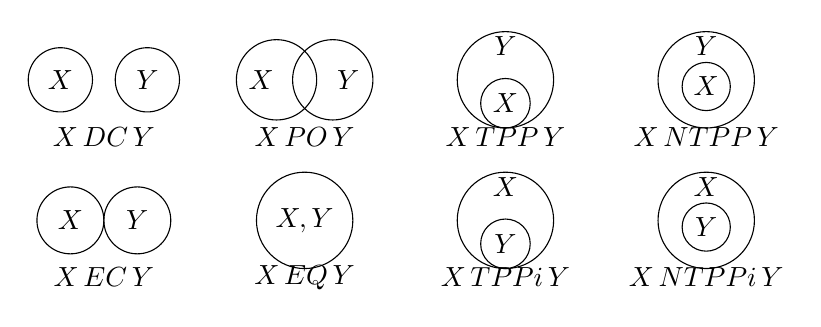
\begin{tikzpicture}[x=1cm,y=1cm,scale=.85]
\begin{scope}
\draw (-.65,.5) circle (.48);\draw (.65,.5) circle (.48);
\node at (-.65,.5) {$X$};\node at (.65,.5) {$Y$};
\node at (0,-.35) {$X\,DC\,Y$};\end{scope}
\begin{scope}[xshift=3cm]
\draw (-.42,.5) circle (.6);\draw (.42,.5) circle (.6);
\node at (-.65,.5) {$X$};\node at (.65,.5) {$Y$};
\node at (0,-.35) {$X\,PO\,Y$};\end{scope}
\begin{scope}[xshift=6cm]
\draw (0,.5) circle (.72);\draw (0,.15) circle (.37);
\node at (0,1) {$Y$};\node at (0,.15) {$X$};
\node at (0,-.35) {$X\,TPP\,Y$};\end{scope}
\begin{scope}[xshift=9cm]
\draw (0,.5) circle (.72);\draw (0,.4) circle (.36);
\node at (0,1) {$Y$};\node at (0,.4) {$X$};
\node at (0,-.35) {$X\,NTPP\,Y$};\end{scope}
\begin{scope}[yshift=-2.1cm]
\draw (-.5,.5) circle (.5);\draw (.5,.5) circle (.5);
\node at (-.5,.5) {$X$};\node at (.5,.5) {$Y$};
\node at (0,-.35) {$X\,EC\,Y$};\end{scope}
\begin{scope}[xshift=3cm,yshift=-2.1cm]
\draw (0,.5) circle (.72);\node at (0,.5) {$X,Y$};
\node at (0,-.35) {$X\,EQ\,Y$};\end{scope}
\begin{scope}[xshift=6cm,yshift=-2.1cm]
\draw (0,.5) circle (.72);\draw (0,.15) circle (.37);
\node at (0,1) {$X$};\node at (0,.15) {$Y$};
\node at (0,-.35) {$X\,TPPi\,Y$};\end{scope}
\begin{scope}[xshift=9cm,yshift=-2.1cm]
\draw (0,.5) circle (.72);\draw (0,.4) circle (.36);
\node at (0,1) {$X$};\node at (0,.4) {$Y$};
\node at (0,-.35) {$X\,NTPPi\,Y$};\end{scope}
\end{tikzpicture}
\caption{Native vector re-presentation of the eight ordinary region
configurations in Ragni's Figure~13.2.1. Circle radius and page position
are illustrative only. The inverse of \(NTPP\) is written \(NTPPi\),
repairing the source caption's transposed-letter spelling.}
\label{fig:p19-rat132-rcc}
\end{figure}

RCC-5 suppresses boundary distinctions: \(DC\) and \(EC\) merge
as discrete regions, \(TPP\) and \(NTPP\) merge as proper part,
and their inverses merge; partial overlap and equality remain. Thus the
five relations are discrete, partial overlap, proper part, inverse proper
part and equality. Whether countries share a border motivates keeping the
RCC-8 distinction. Neither system states which country is north of another.
Uncertain region descriptions again use disjunctions. The chapter mentions
the double-cross calculus, multidimensional interval extensions, robotics,
plan generation, sea navigation and language processing to illustrate
different formal/application domains; these named projects are not
interchangeable complete calculi or evidence that one cognitive account
explains every application.

\section{Six cognitive effects and the source's preferred arrangement}
\label{sec:p19-rat132-effects}

Ragni reviews the following effects, each requiring its original task and
comparison before a quantitative or population-level conclusion is drawn
\cite[sec.~3, pp.~728--729]{Ragni2021SpatialTemporal}.

\paragraph{Indeterminacy.} Descriptions compatible with several scenarios
are often harder than determinate ones in inference tasks. Mental-model
and mental-rule accounts both explain versions of the effect. It is not
a theorem that every multiple-model task is harder: producing \emph{any}
satisfying drawing provides more successful answers when more are allowed.
The primary experiment below makes this contrast concrete.

\paragraph{Relational complexity.} Higher-arity relations such as ternary
between, or information requiring decomposition into simpler relations,
can increase processing difficulty. Number of sentences and relational
arity are not the same measure. A claim about the cost of comparing four
objects is not automatically an effect of storing four independent premises.

\paragraph{Visual impedance.} Easily visualized descriptions can impede
relational inference relative to abstract descriptions. Ragni takes this as
support for an abstract-relational representation rather than a detailed
picture. Image construction followed by extracting relevant relations and
activation of additional declarative features are different proposed
mechanisms. The review does not settle which mechanism uniquely explains
every impedance finding, nor does it say all visual aids harm reasoning.

\paragraph{Continuity.} The source compares \(A<B,B<C,C<D\) in
that order with \(A<B,C<D,B<C\), where \(<\) here means
left-of. Both entail the same linear order; the discontinuous presentation
requires retaining two disconnected pieces before integrating them.
Content equivalence therefore does not imply equal processing demands.

\paragraph{Relevance.} An irrelevant or already-supplied conclusion premise
can make a task easier than one with equally many wholly relevant premises.
The proposed model stores what matters to the query. This is a contextual
claim about the compared tasks, not permission to discard a premise that
changes which countermodels are possible.

\paragraph{Preference.} The source's four car premises state Ferrari left
of Porsche, Beetle right of Porsche, Porsche left of Hummer and Hummer
left of Dodge. With one line and distinct positions they permit these
three orders:
\[
\begin{array}{cl}
1&\text{Ferrari Porsche Beetle Hummer Dodge}\\
2&\text{Ferrari Porsche Hummer Beetle Dodge}\\
3&\text{Ferrari Porsche Hummer Dodge Beetle}.
\end{array}
\]
The chapter calls the first the preferred model and describes higher/faster
acceptance of it than of the second, which in turn is favored over the
third. The question whether Beetle is \emph{necessarily} left of Dodge
exposes the cost of neglecting the third arrangement.

\begin{hbtheorem}{thm:p19-rat132-cars}{proved=annex:p19.rat132.cars}{All three orders, and the preferred-model error}
On one strict linear spatial order with all five cars at distinct positions,
the car premises have exactly the three displayed qualitative orders.
Porsche is necessarily left of Dodge. Beetle left of Dodge is possible
but not necessary; Beetle right of Dodge is also possible. In the graph
whose moves are swaps of adjacent cars preserving the premises, the
three orders form a path \(1\! -\!2\! -\!3\).
Model~3 is two such moves from model~1, not one.
\end{hbtheorem}

This graph is a declared discrete move system, not a theorem forbidding
every conceivable continuous motion in three-dimensional space. Allowing
tied positions adds configurations; allowing another axis changes what
left means. Nothing in the three-order proof measures how likely a person
is to construct one of those orders.

The source also reports that model insertion can be easier for large-scale
cardinal-direction problems than for small-scale left--right arrangements.
This domain comparison is not a consequence of the car-order theorem or
a guarantee for every navigation task. The source describes these effects as repeatedly reported and invokes
cross-cultural similarities and differences, small- and large-scale space,
topological tasks and some other domains. Those are review-level claims
whose individual populations, assignments, estimates and uncertainty are
not supplied in chapter~13.2. They must not be treated as one pooled
experiment, a universal effect size or proof of unrestricted transfer.

\section{PRISM: representation, construction, inspection and variation}
\label{sec:p19-rat132-prism}

Ragni contrasts coordinate-based models with discrete lists/grids,
visual-image architectures such as Casimir, and abstract or verbally
inspired relational accounts. The source's principal computational example
is PRISM, preferred inferences in reasoning with spatial mental models.
Its original presentation specifies five interacting components: input
triples \((X,r,Y)\) naming a located and reference object, abstract object
tokens, a two-dimensional spatial array, a movable focus and a control
process. Here \(X,Y\) name object tokens rather than the planar regions
of the RCC illustration. It presupposes an interpretation of spatial expressions; it does
not implement a natural-language understanding system
\cite[pp.~563--570]{RagniKnauff2013PRISM}.

Construction starts with an empty array. The first-mentioned token of the
first premise is inserted, then the second is placed in the relation's
direction. A subsequent one-new-token premise locates the already
represented reference, then inserts the new token. A two-new-token premise
creates another submodel. A connecting premise groups and integrates
submodels. These distinctions explain why continuous and discontinuous
premise sequences need different operations even when their final premise
sets agree.

If a desired cell is occupied, \emph{first free fit} (fff) proceeds farther
in the indicated direction to a free cell, preserving the placement of
existing tokens. \emph{First fit} (ff) instead relocates tokens to open the
nearest appropriate cell. For Porsche right of Ferrari followed by Beetle
left of Porsche, fff gives Beetle--Ferrari--Porsche while ff gives
Ferrari--Beetle--Porsche. Both obey the premises; the strategy, not the
semantics alone, chooses between them. An annotation records the constrained
token's relation to an anchor so that a later variation can preserve what
the premises actually asserted.

Inspection scans from the last focus position to identify a relation between
queried tokens. Variation starts from the preferred model, using small
changes constrained by annotations. A neighborhood graph organizes nearby
alternatives. Counting focus insertion, movement, refocusing and grouping
operations gives the proposed cognitive-complexity measure. The original
worked continuous/semicontinuous/discontinuous traces count 9, 10 and 12
operations, respectively. These are counts under specified program
conventions, not measured response-time components. Thus the specified
continuous trace has fewer operations than the semicontinuous trace,
which has fewer than the discontinuous trace. Equal operation costs are
an explicit original default
\cite[pp.~566--576,578,584]{RagniKnauff2013PRISM}.

A material qualification concerns the search policy. The 2021 chapter
describes constructing alternatives as counterexample search. The original
2013 PRISM distinguishes variation from systematic validation and expressly
does \emph{not} routinely search for counterexamples when a queried relation
already holds in the preferred model. Variation is particularly triggered
by an explicit all-model request or a relation absent from that model.
This asymmetry helps generate illusory necessity judgments. Correct
normative validation and the model's descriptive search policy must not be
conflated \cite[pp.~568--572,584]{RagniKnauff2013PRISM}.

Likewise, Ragni's resource-bounded interpretation is not an assertion that
the 2013 implementation contains every proposed resource limitation. Its
array capacity is not limited, information-decay is set to zero, and all
focus operations receive equal cost. It omits a belief/knowledge interaction
mechanism and a lexical semantics for fuzzy, intrinsic or viewpoint-dependent
prepositions; it is restricted to two horizontal dimensions, lacks diagonal
reasoning and disallows two tokens in one cell. The operational-parsimony
theory and these implementation defaults have different standing. Simulating
a response pattern shows that a proposed procedure can generate it, not
that the human brain must implement that exact procedure
\cite[pp.~582--585]{RagniKnauff2013PRISM}.

\section{Two primary spatial experiments}
\label{sec:p19-rat132-spatial-evidence}

The original PRISM paper provides experimental checks that are more specific
than the chapter's global preference statement. Its Experiment~1 used
20 Princeton students, nine female, mean age 23.4 years, as their own
controls. Two determinate, two indeterminate one-dimensional and two
indeterminate two-dimensional patterns were each presented twice: twelve
problems, randomized with fruit tokens randomly assigned. Premises were
self-paced, accumulated on screen, then disappeared before participants
drew an arrangement. Multiple drawings were permitted, but neither
requested nor announced as sometimes possible
\cite[pp.~578--579,581, Experiment~1]{RagniKnauff2013PRISM}.

In these reported tests, \(p\) denotes the source's tail-probability
value, not an interval or object token. Correct drawings were reported
for 83 percent of determinate and 92 percent
of indeterminate problems (\(p<.01\)). The authors explain the latter
advantage by the generation task's larger set of correct drawings; it does
not contradict a harder necessary-inference task. In indeterminate problems
the authors report a single drawing in 90 percent of problems; only two participants drew
more than one. Among correct indeterminate drawings, 78 percent followed
fff and 22 percent ff (\(p<.01\)). This conditional denominator is not
78 percent of all trials or all people. The report gives no confidence
intervals, participant-level response table or probability recruitment frame.

Experiment~2 used 25 Freiburg students, eleven female, mean age 23.9 years,
and 24 indeterminate four-premise fruit problems. Half the offered models
were consistent and half inconsistent; the article does not report results
for the inconsistent ones. Premises appeared sequentially, self-paced, each
replacing the previous premise. Participants then judged whether an offered
arrangement was a \emph{possible} model, not whether one relation was
necessary. The consistent alternatives were fff, mixed-strategy and ff
models. Correct acceptance was 92, 81 and 44 percent, respectively. Reported
time comparisons follow the same increasing difficulty order; the printed
numerals are ``3.797 ms'', ``4.359 ms'' and ``6.410 ms''. Their decimal/
thousands convention is not clarified in the report, so these are not
silently converted into calibrated stage durations. The printed trend
tests use Page's \(L\), here a trend-test statistic rather than the
light interval, with \(L=3.55,p<.001\) for error and
\(L=234.5,p<.01\) for response time. No uncertainty intervals or
individual response-time distributions are given
\cite[p.~580, Experiment~2]{RagniKnauff2013PRISM}.

The pattern is consistent with nearby alternatives being easier to recognize,
but acceptance and response time alone do not uniquely establish the exact
sequence of internal swaps. University samples, fruit descriptions, displayed
candidate arrangements, premise visibility and query wording bound the
claims. The 20- and 25-person studies are separate populations and designs;
their results cannot be combined as forty-five independent realizations of
one common task. In particular, accepting a possible arrangement is not
testing a necessary consequence.

\section{Durative temporal reasoning: a distinct primary task}
\label{sec:p19-rat132-temporal-evidence}

Kelly and Khemlani's account represents punctate events by one token when
duration is irrelevant, and durative events by start/end tokens. Its three
principles are iconic structure reflecting chronological order, an intuitive
initial construction versus deliberative revision, and a cost of maintaining
additional models. A discrete model need not depict every timepoint or
encode a ratio between seconds and decades. These are representational
proposals; Allen's thirteen relations were not designed as thirteen primitive
English expressions. ``Starts'' may require a sentence combining equal
beginnings with an earlier ending, and natural-language ``during'' may have
more than one interpretation \cite[pp.~1--3]{KellyKhemlani2019Durative}.

Their illustrative point-order description puts a meeting before a sale,
the sale after a conference, and the meeting before the conference:
meeting--conference--sale. Their durative illustration instead puts the
meeting during the sale and before the conference. The sale can end before
or after the conference; a single initial timeline does not settle this.
This is temporal indeterminacy, not rigid-object rotation.

\begin{hbtheorem}{thm:p19-rat132-durative}{proved=annex:p19.rat132.durative}{The actual alarm/fire/siren contrast}
Interpret during as strict interval containment \(d\), and before as
\(b\), for proper intervals. Alarm during fire and siren before alarm
are consistent both with a siren outside the fire and with a siren during
it. Adding fire during siren makes the premises inconsistent; adding siren
during fire instead makes them consistent. Thus rejecting the latter
description solely because it conflicts with the first chosen arrangement
is not a complete consistency check.
\end{hbtheorem}

The primary experiment recruited 50 native-English-speaking Mechanical Turk
participants for \$2 and a ten-percent chance of a \$10 bonus. Five were
excluded for inappropriate/excessive keypresses or irrelevant debriefing
responses, leaving 45 (21 female, mean age 35). All but six of the original
participants had at most one introductory logic course. It reports a
preregistered prediction and an OSF data locator; this treatment does not
claim to have independently rerun the dataset or audited the preregistration.

Each participant completed sixteen problems, four per cell of a fully
repeated \(2\times2\) design: initial one-model versus multiple-model
patterns, crossed with a consistent versus inconsistent third premise.
Each problem had three relations among three events, beginning with
\(X\) during \(Y\). Comparable-timescale everyday event triplets
avoided strongly punctate events and intended causal associations. Materials
were rotated across structures and order randomized. Participants revealed
premises with the spacebar while earlier premises remained visible, then
pressed f for consistent or j for inconsistent. A practice problem preceded
the task; four open debriefing questions followed it. These visibility and
response conditions differ from PRISM Experiment~2
\cite[pp.~3--4; Appendix]{KellyKhemlani2019Durative}.

Here \(z\) and Cliff's \(\delta\) denote the reported standardized
test statistic and effect-size measure. Reported accuracy was 78 versus
69 percent for one- versus multiple-model
patterns (Wilcoxon \(z=3.02,p=.003\), Cliff's \(\delta=.43\)).
The unadjusted consistency contrast was 72 versus 75 percent
(\(z=1.12,p=.27,\delta=.17\)); this is not equivalence evidence.
The interaction was \(z=4.03,p<.0001,\delta=.42\): consistent
multiple-model problems were particularly difficult, while inconsistent
problems showed little model-number difference. Figure~1's bars are
95-percent confidence intervals, without a printed table of their numerical
endpoints. No response-time result is reported; a theory's speed prediction
must not be relabeled an observed result.

The reported logistic mixed model included the two factors and interaction,
participant intercepts and slopes, and intercepts for items and relation
patterns. Here \(b\) denotes a fitted regression coefficient, not the
before relation. It found a one/multiple contrast
\(b=2.02,z=3.41,p=.0006\), an interaction
\(b=2.35,z=3.21,p=.0013\), and a consistency effect
\(b=1.82,z=4.34,p<.0001\) absent from the unadjusted comparison.
These coefficients belong to that fitted model, not nine-point accuracy
differences or odds ratios reported without a specified contrast coding.
The differing analyses and the unpredicted consistency effect remain visible
\cite[pp.~4--5, fig.~1]{KellyKhemlani2019Durative}.

The authors identify three limits: some participants reported pattern-based
strategies; errors do not reveal whether alternatives were never attempted
or attempted unsuccessfully; and the sixteen three-event structures give
only four problems per cell. A broader interpretation of during as overlap
changes some normative labels. It cannot make an already-consistent strict-
containment description inconsistent, but may make some labeled inconsistent
ones consistent. Accordingly, the particularly poor consistent-multiple
performance survives that particular semantic objection, without proving
that all labels, all ``while'' problems or a general temporal mechanism are
validated. The single experiment is neither a cross-cultural replication
nor an intervention showing that training transfers to navigation
\cite[pp.~5--6]{KellyKhemlani2019Durative}.

\section{Neural, content and rationality boundaries}
\label{sec:p19-rat132-limits}

Ragni's neural review separates frontal control/premise integration from
parietal representation and highlights superior parietal involvement.
It refers to the 47-fMRI-study Wertheim--Ragni meta-analysis, describing
frontal Brodmann areas~6 and~45 and parietal area~7. It also reports a
2016 TMS study: disruption of superior parietal processing reduced preferred-
model construction without a reported comparable reduction for alternatives,
and working-memory capacity moderated susceptibility. These remain the
chapter's review reports. Chapter~13.2 gives neither the TMS sample and
full stimulation/control protocol nor the effect estimates and uncertainty
needed to establish those original causal/localization claims here.
The cross-linked neural treatment in
\cref{sec:p19-rationality-1-4} distinguishes convergent evidence from
one-to-one mapping of a reasoning process to a brain region. Neither a
regional association nor a selective reported null proves a monolithic
storage module or complete independence of construction and variation
\cite[sec.~4, p.~729]{Ragni2021SpatialTemporal}.

Content, background beliefs and embodied response arrangements also matter
in the chapter's argument. A familiar silverware arrangement may guide
the initial model. Its SNARC discussion contrasts faster left-hand responses
to smaller numbers with faster right-hand responses to larger ones, then
reports a related spatial-relation/response-side effect. These are bounded
review illustrations, not a finding that all cultures, handedness groups
or every numerical and spatial task share a fixed left--right mental axis.
The source's conclusion that embodiment matters does not identify the
representational mechanism uniquely \cite[secs.~5--6]{Ragni2021SpatialTemporal}.

The source's blood-relatedness example makes the danger of indiscriminate
transitivity concrete: a father and daughter are blood-related, as are the
daughter and mother, but the parents need not be blood-related to one
another. The transitivity theorem for an ordered spatial axis cannot be
transferred to this symmetric but nontransitive relation. A linear mental
layout may explain an erroneous answer; it does not repair that answer's
logic. Likewise, RCC contact, interval overlap and ``is a relative of''
must not acquire transitivity just because before and northward order have it.

Ragni defends preferred-model parsimony as sensible under limited time,
working memory and computing resources, and suggests that finding an optimal
path or time plan may cost more than everyday purposes require. This is
a process-sensitive bounded-rationality argument. It does not alter the
formal distinction between possible and necessary, specify a universal
resource budget, supply an empirical utility function, or prove that every
observed error is optimal. When a wrong route, missed deadline or false
necessary inference has high consequences, the saved effort must be compared
with those losses and with available alternatives. Explaining a systematic
error and recommending the mechanism are different claims
\cite[secs.~6.3--7, pp.~731--732]{Ragni2021SpatialTemporal}.

For consultation, choose a relation benchmark matching the question.
Use one model to witness possibility; use a countermodel to refute necessity;
use a complete procedure or justified invariant to establish necessity or
inconsistency. Respect endpoint equality, boundary contact, query wording,
premise visibility and the declared frame. The car-order and durative
examples supply actual success/failure cases; a nonempty propagation fixed
point, a favored arrangement or an unqualified transitivity heuristic
supplies no general validity certificate.

\Cref{sec:p19-mental-rotation} instead studies congruence after a rigid
transformation, arbitrary feature bindings, response times and eye movements.
Its visual-transform evidence does not discharge relational-inference
claims. \Cref{sec:p12-rationality-13-1} treats external diagram syntax,
semantics and sound transformations; an Euler free ride valid in every
interpretation is not the extra left--right relation of one preferred
internal model. Both comparisons preserve the distinction between a
representation's normative meaning and its processing properties. The
empirical-record discipline of \cref{def:p19-evidence-record} applies
separately to the spatial and temporal studies. No missing original TMS,
cross-cultural, visual-impedance or response-side evidence record is filled
by borrowing the populations or estimates of the primary experiments above.
